\begin{pa} \label{PA:9.3}
  For two-dimensional vectors $\vu=\langle u_1,u_2\rangle$ and
  $\vv=\langle v_1, v_2\rangle$, the dot product is simply the scalar
  obtained by
  $$
  \vu\cdot\vv = u_1v_1 + u_2v_2.
  $$

    \ba
  \item If $\vu=\langle 3, 4\rangle$ and $\vv=\langle -2, 1\rangle$,
    find the dot product $\vu\cdot\vv$.

  \item Find $\vi\cdot\vi$ and $\vi\cdot\vj$.

  \item If $\vu=\langle 3, 4\rangle$, find $\vu\cdot\vu$.  How is this
    related to $|\vu|$?

  \item On the axes in Figure \ref{F:9.3.preview.1}, plot the
    vectors $\vu=\langle 1, 3\rangle$ and $\vv=\langle -3, 1\rangle$.  Then, 
    find $\vu\cdot\vv$.  What is the angle between these vectors?  

    \begin{figure}[ht]
      \begin{center}
        \includegraphics{figures/fig_9_3_preview_1.eps}
        \caption{For part (d)}
        \label{F:9.3.preview.1}
      \end{center}
    \end{figure}

  \item On the axes in Figure \ref{F:9.3.preview.2}, plot the
    vector $\vu=\langle 1, 3\rangle$.

    \begin{figure}[ht]
      \begin{center}
        \includegraphics{figures/fig_9_3_preview_1.eps}
        \caption{For part (e)}
        \label{F:9.3.preview.2}
      \end{center}
    \end{figure}

    For each of the following vectors $\vv$, plot the vector on Figure
    \ref{F:9.3.preview.2} and then compute the dot product
    $\vu\cdot\vv$. 

    \begin{itemize}
      \item $\vv=\langle 3, 2 \rangle$.
      \item $\vv=\langle 3, 0 \rangle$.
      \item $\vv=\langle 3,-1 \rangle$.
      \item $\vv=\langle 3,-2 \rangle$.
      \item $\vv=\langle 3,-4 \rangle$.
      \end{itemize}

    \item Based upon the previous part of this activity, what do you
      think is the sign of the dot product in the following three
      cases shown in Figure \ref{F:9.3.preview.3}?

    \begin{figure}[ht]
      \begin{center}
        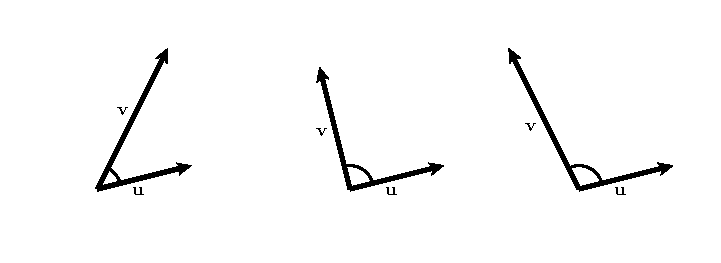
\includegraphics{figures/fig_9_3_preview_2.eps}
        \caption{For part (f)}
        \label{F:9.3.preview.3}
      \end{center}
    \end{figure}

      


    \ea

\end{pa} 

\begin{activitySolution}
    \ba
  \item Here we have $u_1=3$, $u_2=4$, $v_1=-2$, and $v_2=1$, so 
\[\vu \cdot \vv = \langle 3, 4\rangle \cdot \langle -2, 1\rangle = (3)(-2)+(4)(1) = -2.\]

  \item Since $\vi = \langle 1,0 \rangle$ and $\vj = \langle 0,1 \rangle$, it follows that 
\[\vi\cdot\vi = 1 \ \text{ and } \ \vi\cdot\vj = 0.\]

  \item In this case we have 
\[\vu \cdot \vu = \langle 3, 4\rangle \cdot \langle 3, 4\rangle = 3^2+4^2 = 25.\]
By the distance formula, the length of $\vu$ is 
\[|\vu| = \sqrt{3^2+4^2} = 5.\]
So $\vu \cdot \vu = |\vu|^2$. 

  \item The slope of the line through the origin and the point $(1,3)$ is 1 while the slope of the line through the origin and the point $(-3,1)$ is $-\frac{1}{3}$. Since these slopes are negative reciprocals, the lines are perpendicular. Thus, the angle between $\vu$ and $\vv$ is $90^{\circ}$. Also
\[\vu \cdot \vv = \langle 1, 3\rangle \cdot \langle -3, 1\rangle = (1)(-3)+(3)(1) = 0.\]

  \item With $\vu=\langle 1, 3\rangle$ we have 
    \begin{itemize}
      \item $\vu \cdot \langle 3, 2 \rangle = \langle 1, 3\rangle \cdot \langle 3, 2 \rangle = 9$.
      \item $\vu \cdot \langle 3, 0 \rangle = \langle 1, 3\rangle \cdot \langle 3, 0 \rangle = 1$.
      \item $\vu \cdot \langle 3, -1 \rangle = \langle 1, 3\rangle \cdot \langle 3, -1 \rangle = 0$.
      \item $\vu \cdot \langle 3, -4 \rangle = \langle 1, 3\rangle \cdot \langle 3, -4 \rangle = -9$.
      \end{itemize}

    \item If two vectors are perpendicular, it appears that their dot product is 0. If the vectors form an acute angle (less than $90^{\circ}$ as with $\vu$ and $\langle 3,2 \rangle$ or $\langle 3,0 \rangle$ from the previous part of this activity), then it looks as though their dot product is positive. Finally, if the vectors form an obtuse (greater than $90^{\circ}$ as with $\vu$ and $\langle 3,-4 \rangle$ from the previous part of this activity), then it looks as though their dot product is negative. 
    \ea
\end{activitySolution}

\afterpa 